\liti 一队学生去校外进行军事野营训练。 他们以 5 千米/时(即 5 千米每小时)的速度行进,走了 18 分的时候,
学校要将一紧急通知传给队长。 通讯员从学校出发,骑自行车以 14 千米/时 的速度按原路追上去。
通讯员用多少时间可以追上学生队伍?

分析:在这个问题里,当通讯员追上学生队伍时,通讯员和学生队伍所走的路程是相同的。

在通讯员追赶前的 18 分内,学生队伍走的路程是可以求出的。
如果设通讯员追上学生队伍需要 $x$ 小时, 那么由于他们的速度都是已知的,
在这段时间里走的路程都可以表示出来(图 \ref{fig:3-5}),从而可以按照上面的相等关系列出方程。

\begin{figure}[htbp]
    \centering
    \begin{tikzpicture}
    \pgfmathsetmacro{\a}{0}
    \pgfmathsetmacro{\b}{5.5}
    \pgfmathsetmacro{\c}{7}

    \draw [ultra thick] (\a, 0) -- (\c, 0);
    \foreach \x in {\a, \b, \c} {
        \draw (\x, 0.2) -- (\x, -0.2);
    }
    \draw[decorate, decoration={brace, amplitude=0.3cm}] (\a, 0.3) -- (\c, 0.3)
        node [pos=0.5, above=1em, align=center] {$14x$};
    \draw[decorate, decoration={brace,mirror, amplitude=0.3cm}] (\a, -0.3) -- (\b, -0.3)
        node [pos=0.5, below=1em, align=center] {$5 \times \dfrac{3}{10}$};
    \draw[decorate, decoration={brace,mirror, amplitude=0.3cm}] (\b, -0.3) -- (\c, -0.3)
        node [pos=0.5, below=1em, align=center] {$5x$};
\end{tikzpicture}

    \caption{}\label{fig:3-5}
\end{figure}

\begin{enhancedline}
\jie 设通讯员用 $x$ 小时可以追上学生队伍, 那么通讯员走了 $14x$ 千米;
学生队伍在被追赶前的 18 分内先走了 $\left(5 \times \dfrac{3}{10}\right)$ 千米,
在以后的 $x$ 小时内又走了 $5x$ 千米。 根据题意,得
$$ 14x = 5 \times \dfrac{3}{10} + 5x \juhao $$

解这个方程:
\begin{align*}
    9x &= \dfrac{3}{2} \douhao \\
    x  &= \dfrac{1}{6} \juhao
\end{align*}

答: 通讯员用 10 分可以追上学生队伍。
\end{enhancedline}


\liti 一件工作, 甲单独做 20 小时完成, 乙单独做 12 小时完成。
现在先由甲单独做 4 小时, 剩下的部分山甲、乙合做。 剩下的部分需要几小时完成?

分析: 我们把全部工作量看成 1。 由于甲、乙分别做完全部工作的时间是已知的,
他们每小时完成的工量也是已知的。 如果设剩下的部分需要 $x$ 小时完成,
那么甲先在 4 小时内完成的工作量, 合做时甲、乙分别完成的工作量都可以表示出来。
根据 “这三部分工作量的和等于全部工作量” (图 \ref{fig:3-6}),就可以列出方程。

\begin{figure}[htbp]
    \centering
    \begin{tikzpicture}
    \pgfmathsetmacro{\a}{0}
    \pgfmathsetmacro{\b}{2}
    \pgfmathsetmacro{\c}{5}
    \pgfmathsetmacro{\d}{10}

    \draw [ultra thick] (\a, 0) -- (\d, 0);
    \foreach \x in {\a, \b, \c, \d} {
        \draw (\x, 0.2) -- (\x, -0.2);
    }
    \draw[decorate, decoration={brace, amplitude=0.3cm}] (\a, 0.3) -- (\d, 0.3)
        node [pos=0.5, above=1em, align=center] {全部工作量 \\ 1};
    \draw[decorate, decoration={brace,mirror, amplitude=0.3cm}] (\a, -0.3) -- (\b, -0.3)
        node [pos=0.5, below=1em, align=center] {$\dfrac{4}{20}$ \\[.5em] 甲先单独完 \\ 成的工作量};
    \draw[decorate, decoration={brace,mirror, amplitude=0.3cm}] (\b, -0.3) -- (\c, -0.3)
        node [pos=0.5, below=1em, align=center] {$\dfrac{x}{20}$ \\[.5em] 合做时甲完 \\ 成的工作量};
    \draw[decorate, decoration={brace,mirror, amplitude=0.3cm}] (\c, -0.3) -- (\d, -0.3)
        node [pos=0.5, below=1em, align=center] {$\dfrac{x}{12}$ \\[.5em] 合做时乙完 \\ 成的工作量};
\end{tikzpicture}

    \caption{}\label{fig:3-6}
\end{figure}

\jie 设甲、乙两人合做剩下的部分需要 $x$ 小时完成, 那么当把全部工作量看成是 1 时,
甲先在 4 小时内完成的工作量是 $\dfrac{4}{20}$,
合做时甲、乙完成的工作量分别是 $\dfrac{x}{20}$ 与 $\dfrac{x}{12}$。
根据题意,得
$$ \dfrac{4}{20} + \dfrac{x}{20} + \dfrac{x}{12} = 1 \juhao $$

解这个方程:
\begin{align*}
    12 + 3x + 5x = 60 \douhao \\
    8x = 48 \douhao \\
    x = 6 \juhao
\end{align*}

答: 甲、乙两人合做剩下的部分需要 6 小时完成。


\lianxi
\begin{xiaotis}

列出一元一次方程解下列应用题:

\xiaoti{甲、乙两人练习短距离赛跑, 甲每秒跑 7 米, 乙每秒跑 6.5 米。 如果甲让乙先跑 1 秒, 甲经过几秒可以追上乙?}

\xiaoti{甲、乙两人从同地出发去某地。 甲步行,每小时走 5 千米, 先走1.5 小时;乙骑自行车。
    乙走了 50 分, 两人同时到达目的地。乙每小时走多少千米?
}

\xiaoti{某地下管道由甲工程队单独铺设需 12 天, 由乙工程队单独铺设需18 天。
    如果由这两个工程队从两端同时相向施工,要多少天可以铺好?
}

\xiaoti{某工作甲单独做 3 小时完成, 乙单独做 5 小时完成。
    两人合做这项工作的 $\dfrac{4}{5}$, 需要几小时完成?
}

\xiaoti{某单位分三期完成一项工程。 第一期用了全部工程时间的 $40\%$,
    第二期用了全部工程时间的 $36\%$, 第三期工程用了 24 天。完成全部工程共用了多少天?
}

\end{xiaotis}
\lianxijiange


\liti 要用含氨 $0.15\%$ 的氨水进行油菜追肥。 现有含氨 $16\%$ 的氨水 30 千克,配制时需要加水多少千克?

分析:氨水加水后,重量和浓度都发生了变化,但氨水中所含氨的重量没有变化(图 \ref{fig:3-7})。也就是有等式:
$$ \text{加水前含氨重量} = \text{加水后含氨重量} \juhao $$

\begin{figure}[htbp]
    \centering
    \begin{tikzpicture}
    \tikzset{
        rongye/.style={
            left color=gray!50,
            right color=gray!30,
            middle color=white,
            fill opacity=0.6,
        },
        shaobei/.pic={
            \pgfmathsetmacro{\h}{#1}
            \path[rounded corners=2pt, rongye]
                (0.1, -1.95 + \h) -- (0.1, -1.95)
                -- (1.9, -1.95) -- (1.9, -1.95 + \h) -- cycle;
            % 下一行是为了消除填充色上部的圆角
            \path[rongye] (0.1, -1.95 + \h) rectangle (1.9, -1.95+\h-0.05);

            \draw [rounded corners=2pt]
                    (0, 0) -- (0.05, -0.1) -- (0.05, -2)
                -- (1.95, -2) -- (1.95, -0.1) -- (2.0, 0);
            \draw [rounded corners=2pt] (0, 0) -- (0.1, -0.1) -- (0.1, -1.95)
                -- (1.9, -1.95) -- (1.9, -0.1) -- (2.0, 0);
            \draw (0, 0) -- (2, 0);
        }
    }

    \begin{scope}
        \draw (0, 0) pic {shaobei = 0.4};
        \foreach \x/\y in {
            0.2/-1.85, 0.3/-1.8, 0.5/-1.75,
            0.8/-1.85, 1.0/-1.7, 1.2/-1.85,
            1.4/-1.75, 1.6/-1.8, 1.8/-1.75
        } {
            \draw (\x, \y) circle(0.03);
        }
        \node at (1, -2.4) {$16\%$ 氨水};
        \node at (1, -2.8) {30 千克};
    \end{scope}

    \node at (4, -0.6) {加水 $x$ 千克后};
    \draw [fill=white] (3.5, -1.1) pic [rotate=-90] {arrow={.2}{.6}{.4}{.2}};
    \draw (3, -2.5) circle(0.03) node [right] {示意含氨量};

    \begin{scope}[xshift=6cm]
        \draw (0, 0) pic {shaobei = 1.5};
        \foreach \x/\y in {
            0.9/-1.6, 1.5/-1.6, 0.4/-1.3,
            1.3/-1.25, 0.8/-1.0, 1.6/-1.0,
            0.6/-0.8, 1.0/-0.7, 1.8/-0.8
        } {
            \draw (\x, \y) circle(0.03);
        }
        \node at (1, -2.4) {$0.15\%$ 氨水};
        \node at (1, -2.8) {$(30 + x)$ 千克};
    \end{scope}
\end{tikzpicture}

    \caption{}\label{fig:3-7}
\end{figure}

由于重量和浓度都是已知的, 加水前含氨的重量就可以求得。
另外, 因为加水后的浓度已知, 所以如果设需要加水 $x$ 千克,
那么可以表示出加水后氨水的重量和氨水中含氨的重量, 从而可以按照上面的相等关系列出方程。

\begin{enhancedline}
\jie 设需要加水 $x$ 千克, 那么加水后氨水重量是 $(30 + x)$千克,
氨水中含氨重量是 $(30 + x) \times 0.15\%$ 千克;
加水前氨水中含氨重量是 $30 \times 16\%$千克。
根据题意,得
$$ (30 + x) \times \dfrac{0.15}{100} = 30 \times \dfrac{16}{100} \juhao $$
\end{enhancedline}

解这个方程:
\begin{align*}
    0.15 (30 + x) &= 30 \times 16 \douhao \\
    30 + x &= 3200 \douhao \\
    x &= 3170 \juhao
\end{align*}

答: 需要加水 3170 千克 。


\begin{enhancedline}
\liti 一个两位数, 十位上的数比个位上的数小 1 , 十位上的数与个位上的数的和是这个两位数的 $\dfrac{1}{5}$,求这个两位数。

分析:因为已知十位上的数比个位上的数小 1 , 所以如果设十位上的数为 $x$,就可以写出个位上的数,
从而可以写出 “两个数位的数的和” 与这个两位数。
根据 “两个数位的数的和等于这个两位数的 $\dfrac{1}{5}$”, 就可以列出方程。

\jie 设十位上的数为 $x$,那么个位上的数是 $x + 1$ ,
它们的和是 $x + (x + 1)$, 这个两位数是 $10x + (x + 1)$,
根据题意,得
$$ x + (x + 1) = \dfrac{1}{5}[10x + (x + 1)] \juhao $$
\end{enhancedline}

解这个方程:
\begin{align*}
    2x + 1 &= \dfrac{1}{5}(11x + 1) \douhao \\
    10x + 5 &= 11x + 1 \douhao \\
    x &= 4 \douhao \\
    x + 1 &= 5 \juhao
\end{align*}

答:所求的两位数为 45 。


\lianxi
\begin{xiaotis}

\xiaoti{直接写出:}
\begin{xiaoxiaotis}

    \xxt{含盐 $6\%$ 的盐水 10 千克,其中含盐多少千克?}

    \xxt{含盐 $10\%$ 的盐水 $x$ 千克,其中含盐多少千克?}

\end{xiaoxiaotis}

列出一元一次方程解下列应用题:

\xiaoti{有含盐 $15\%$ 的盐水 20 千克,要使盐水含盐 $10\%$,需要加水多少千克?}

\xiaoti{有含盐 $15\%$ 的盐水 20 千克,要使盐水含盐 $20\%$,需要加盐多少千克?}

\xiaoti{一个两位数,个位上的数是十位上的数的 2 倍, 如果把十位上的数与个位上的数对调,
    那么所得到的两位数比原两位数大 36, 求原两位数。
}

\xiaoti{长方形的周长为 16 米,长比宽多 2 米,求它的面积。}

\end{xiaotis}

